% this file is part of the Stellar Spectroscopy project
% Copyright 2013 2014 the authors

\documentclass[manuscript]{aastex}
\usepackage{graphicx}
\shorttitle{Title[INSERT]}
\shortauthors{Mei \& Hogg}



\begin{document}

\title{Longer Title[INSERT]}

\author{M. J. Mei\altaffilmark{1}}
\affil{New York University Abu Dhabi, PO Box 129188, Abu Dhabi, UAE}

\author{David W. Hogg\altaffilmark{2,3}}
\affil{Center for Cosmology and Particle Physics, Department of Physics, New York University, 4 Washington Place, New York, NY 10003, USA}


\altaffiltext{1}{New York University Abu Dhabi, PO Box 129188, Abu Dhabi, UAE}
\altaffiltext{2}{Center for Cosmology and Particle Physics, Department of Physics, New York University, 4 Washington Place, New York, NY 10003, USA}
\altaffiltext{3}{Max-Planck-Institut f{\"u}r Astronomie, Konigst{\"u}hl 17, D-69117 Heidelberg, Germany}


\begin{abstract}
[INSERT] Abstract
\end{abstract}

\keywords{luminosity modelling, extinction, equivalent width}

\section{Introduction}

\section{Data}
\subsection{Querying SDSS (DR9)}

- This seeks the standard (calibration) stars as defined on SDSS's "Algorithms" webpage:\\  \url{http://www.sdss3.org/dr9/algorithms/boss\_std\_ts.php}. 
- There is one modification: instead of \\ $\sqrt{((u-g)-0.82)^2+((g-r)-0.3)^2+((r-i)-0.09)^2+((i-z)-0.02)^2}<0.08$ we used $|(u-g)-0.82|<0.08$, $|(g-r)-0.3|<0.08$ etc. \\
- The output gives the extinction (in the g-band), the recorded flux, equivalent width and continuum values given in galSpecLine for the H-$\alpha$, H-$\beta$, H-$\gamma$, H-$\delta$ lines. \\
- However, due to the reported equivalent widths being unreasonable compared to manual estimations, the query also extracts the plate-mjd-fiber values and downloads, via wget, the relevant FITS file for this plate-mjd-fiber combination. \\
- The full query is here: 
\begin{verbatim}"SELECT p.objID, p.extinction_g, s.elodieTEff, p.extinction_g,
 p.extinction_g, p.extinction_g, p.extinction_g, p.extinction_g,
 p.obj, s.plate, s.fiberID, s.mjd, g.h_alpha_flux, g.h_alpha_reqw, 
 p.psfMag_u, p.psfMag_g, p.psfMag_r, p.psfMag_i, p.psfMag_z 
    FROM PhotoObj AS p 
    JOIN SpecObj as s ON s.specobjID=p.specobjID 
    WHERE psfMag_r BETWEEN 15.0 and 19.0 
    AND p.type=6 AND  dbo.fPhotoStatus('PRIMARY')>0 AND 
dbo.fPhotoFlags('STATIONARY')>0  and  calibStatus_r=1 
AND s.elodieTEff!=0 AND s.elodieFeH!=0 AND s.elodieLogG!=0 
 AND  ((flags&dbo.fPhotoFlags('BLENDED')) 
 +(flags&dbo.fPhotoFlags('DEBLEND_TOO_MANY_PEAKS')) +   
(flags&dbo.fPhotoFlags('SATURATED')) +
(flags&dbo.fPhotoFlags('BADSKY')) + 
(flags&dbo.fPhotoFlags('COSMIC_RAY')) +
(flags&dbo.fPhotoFlags('PEAKS_TOO_CLOSE')) +   
(flags&dbo.fPhotoFlags('NOTCHECKED_CENTER')) +
(flags&dbo.fPhotoFlags('SATUR_CENTER')) +  
(flags&dbo.fPhotoFlags('INTERP_CENTER')) +
(flags&dbo.fPhotoFlags('INTERP'))+  
(flags&dbo.fPhotoFlags('PSF_FLUX_INTERP')))=0 
    AND  (psfMag_u-psfmag_g) between 0.82-0.08 and 0.82+0.08 
    AND (psfMag_g-psfmag_r) between 0.3-0.08 and 0.30+0.08 
    AND (psfMag_r-psfmag_i) between 0.09-0.08 and 0.09+0.08 
    AND (psfMag_i-psfmag_z) between 0.02-0.08 and 0.02+0.08 
    ORDER BY extinction_g DESC"\\
\end{verbatim}
- There are 11254 stars.
\subsection{Redshift correction}
- The wavelengths were corrected for redshift using the value recorded from HDU2 (copy of SpecObj table from SDSS).\\
\begin{figure}
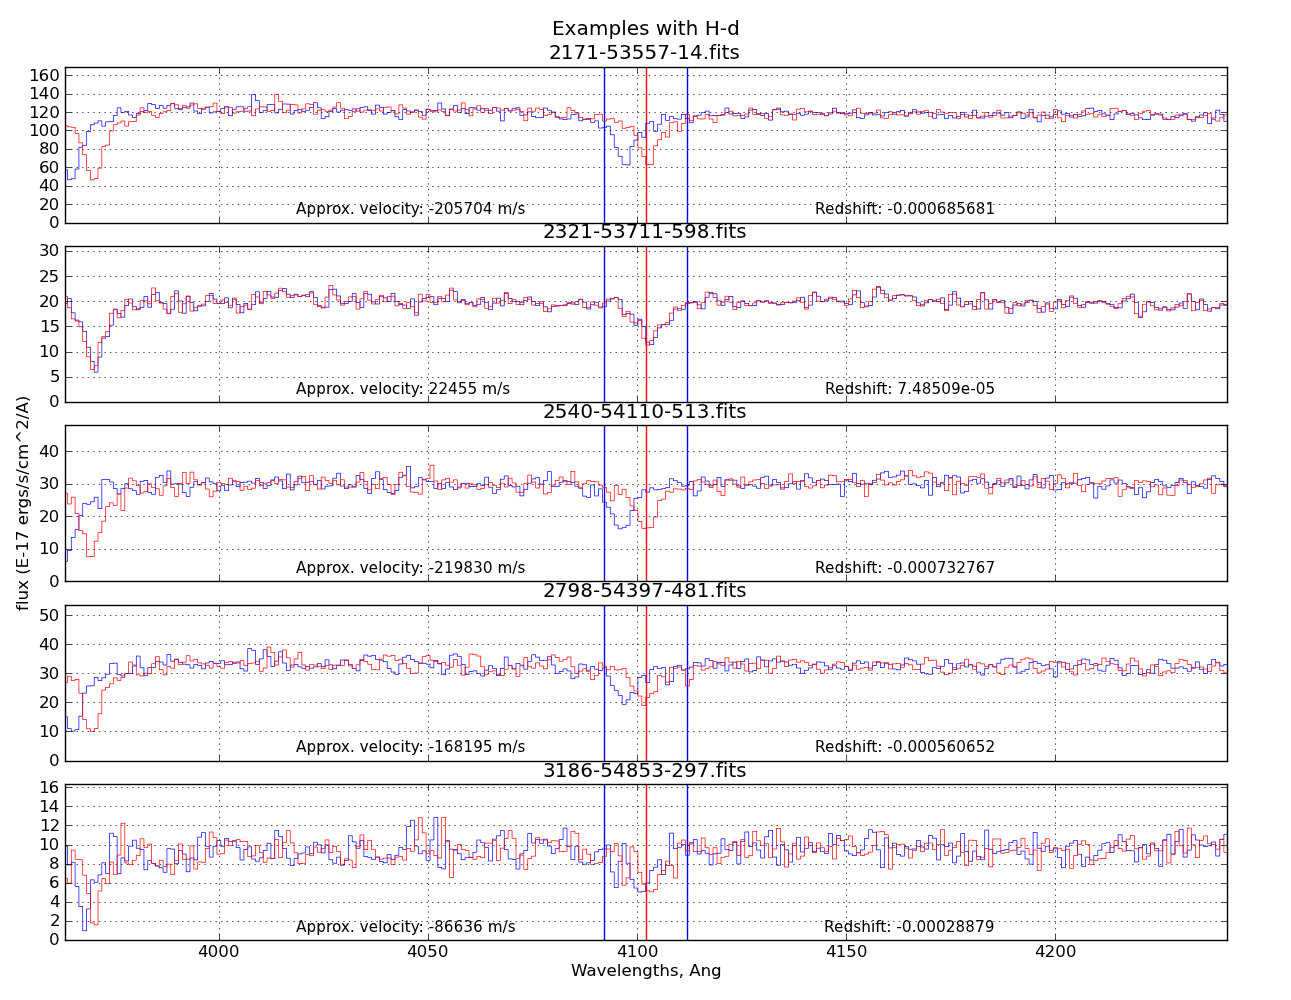
\includegraphics[width=8cm]{../splines_correct}\\
\caption{Red line shows redshift correction; blue shows the reversed correction.}
\end{figure}

\begin{figure}
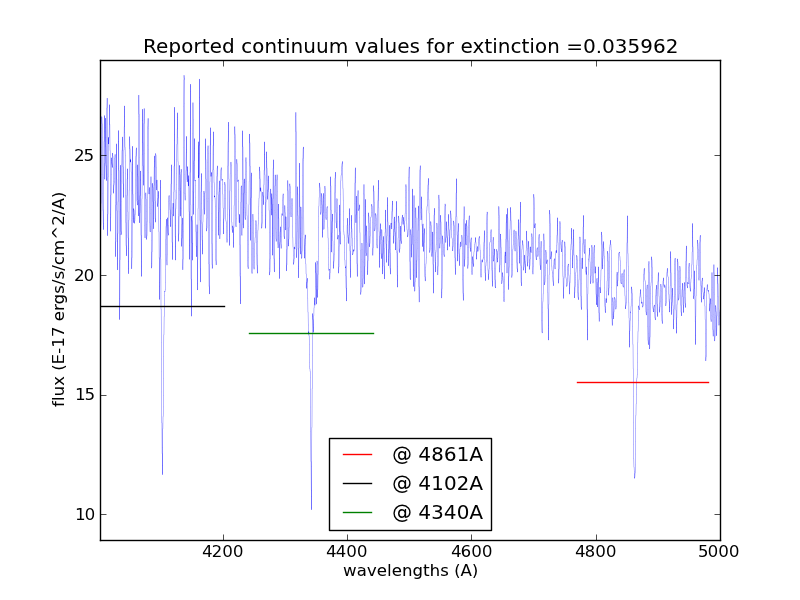
\includegraphics[width=8cm]{../035}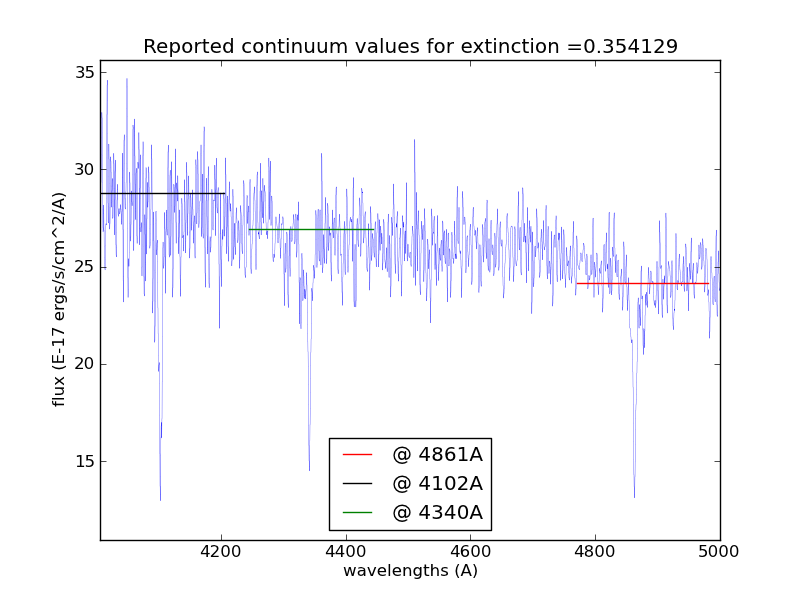
\includegraphics[width=8cm]{../355}\\
\caption{The recorded continuum values in GalSpecLine seem to be only valid for high (above 0.25) extinction values.}
\end{figure}

\section{Methods and Results}
\subsection{Generating new continuum, flux and equivalent-width values}
- The equivalent width is defined by the width such that the area of a rectangle with a height of the continuum value is equal to the area in a spectral line.\\
- We want to use equivalent widths because they essentially measure flux in units of continuum. This means it gives the fraction of light absorbed, instead of the actual number of photons. This means that even if two stars are of different brightness, if viewed through the same interstellar medium (e.g. dust) they will have similar equivalent widths. Moreover, the equivalent width is independent of instrumental resolution and so allows for low-resolution spectra to be used.\\
- However, the calibration of the spectra is suspect - the atmosphere might be introducing unknown wavelength-dependent multiplicative factors, so new values need to be generated using the SDSS spectra.\\
- The spectra are first corrected for redshift.\\
- A cubic spline is used to interpolate the spectrum over a common rest-wavelength grid.\\
- Near the location of each peak, a neighborhood of $\pm$100$\AA$ is taken, excluding a $\pm$10$\AA$ neighborhood (which will be used for flux integration) and the median of this is taken as the continuum, and a $\pm$10$\AA$ neighborhood is taken as the domain for the flux integration.\\
- The flux is numerically integrated over this 20$\AA$ range, using the trapezium rule with a step size of  $\frac{max(\lambda)-min(\lambda)}{10*n(\lambda)}$, and the ratio of flux/continuum gives the equivalent width value.\\
- Each calculation gives an output of a list [continuum, continuum error, flux, flux error, equivalent width, extinction$_g$, plate, mjd, fiber]. This is repeated for all the relevant peaks for each spectra; then this is repeated for all the absorption lines used and collected into one array. This array is sorted first by spectral line then by spectra. It can also be stored in a binary text file using the "pickle" module. \\
\begin{figure}
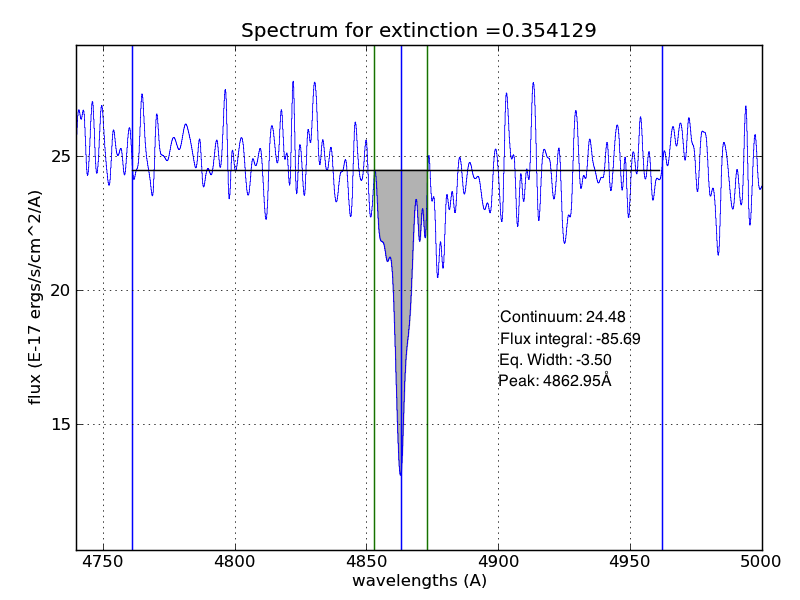
\includegraphics[width=8cm]{../workingexample}\\
\caption{This shows the continuum and equivalent-width estimation. The green lines are each 10$\AA$  away from the central blue line. The blue lines in the extreme left and right are defined at 4761$\AA$ and 4962$\AA$  respectively. The shaded gray area is the flux and the black horizontal line is the continuum.}
\end{figure}
\begin{figure}
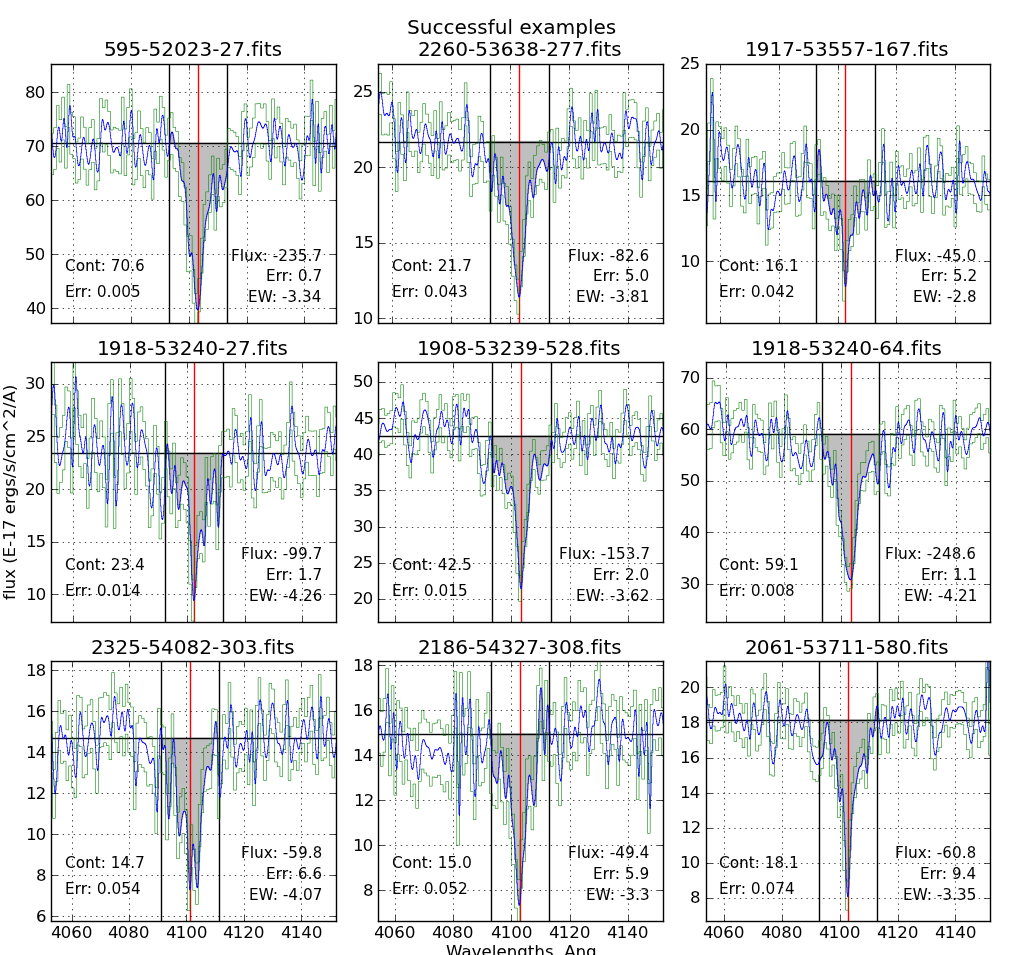
\includegraphics[width=10cm]{../success_labeled}\\
\caption{Example calculations for spectra.}
\end{figure}
\begin{figure}
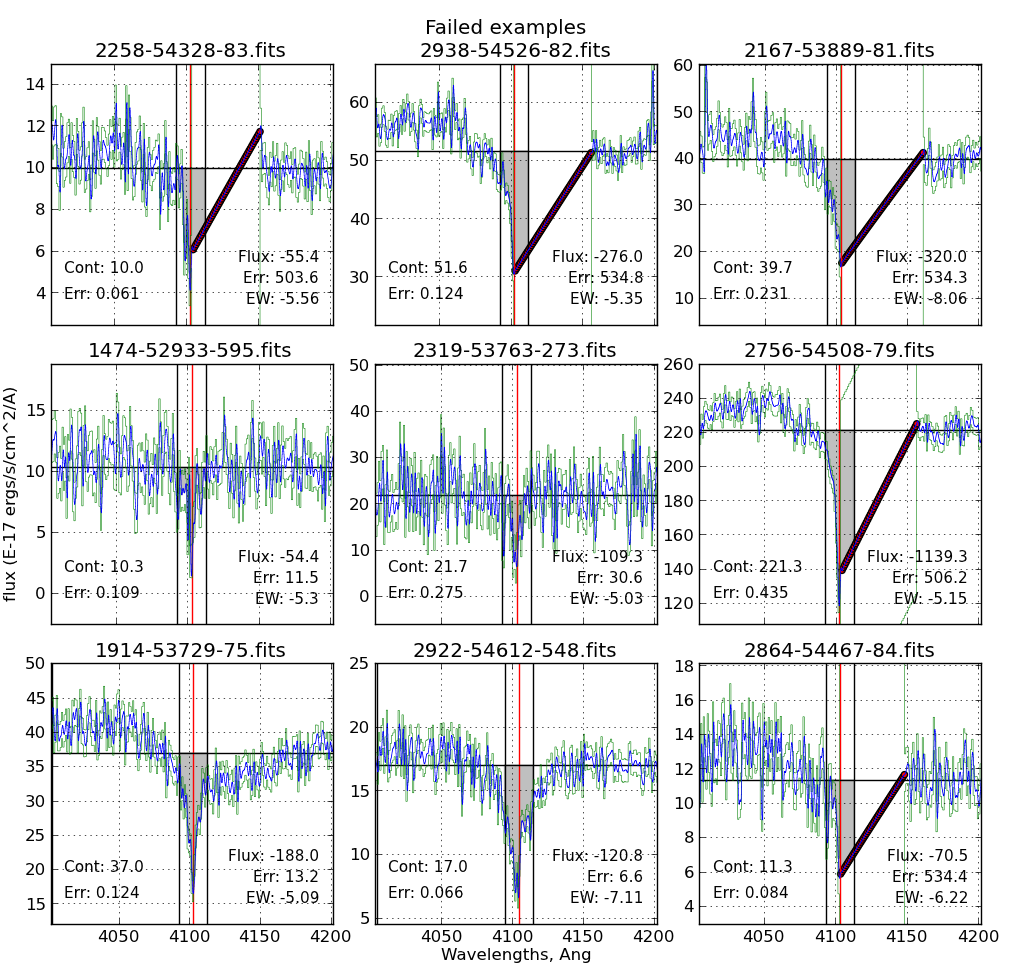
\includegraphics[width=8cm]{../failb_labeled}\\
\caption{Noted failures: varying reasons lead to an overestimate of the flux and consequentially, equivalent width. The main sources are (1) a sudden jump in flux values; (2) a particularly noisy spectrum which leads to a lot of flux from the wings being included; (3) the continuum being not very flat which means more there is more flux between the continuum line and spectrum.}
\end{figure}

\subsection{Fitting flux as a linear function of H-$\delta$ EW, Extinction and Brightness}
- At each particular wavelength, all the flux, H-delta EW, extinction (g), and g-band magnitude were collected. \\
- A linear model was fitted to find three coefficients:\\
Observed flux = a $\times$ Brightness + b $\times$ H-$\delta$  EW + c $\times$ Extinction

 where brightness = 10$^{-0.4 \times (mag_g - 22.5)}$\\
- The fit was done using the scipy.optimize.curve\_fit module, which minimizes the sum of squares of the target function (in this case $\sqrt{ivar}$ $\times$ $|f(B,H,E)-flux|$).
\\
- These coefficients were different for each wavelength, and a plot of each coefficient as a function of wavelength was plotted.\\
- The square root of the main diagonal of the covariance matrix of the fitted parameters is used as the error for the fits. These are stored via the pickle module.\\
- The Balmer lines, known DIBs and telluric lines were plotted as well to see if these affected the fit.

\begin{figure}
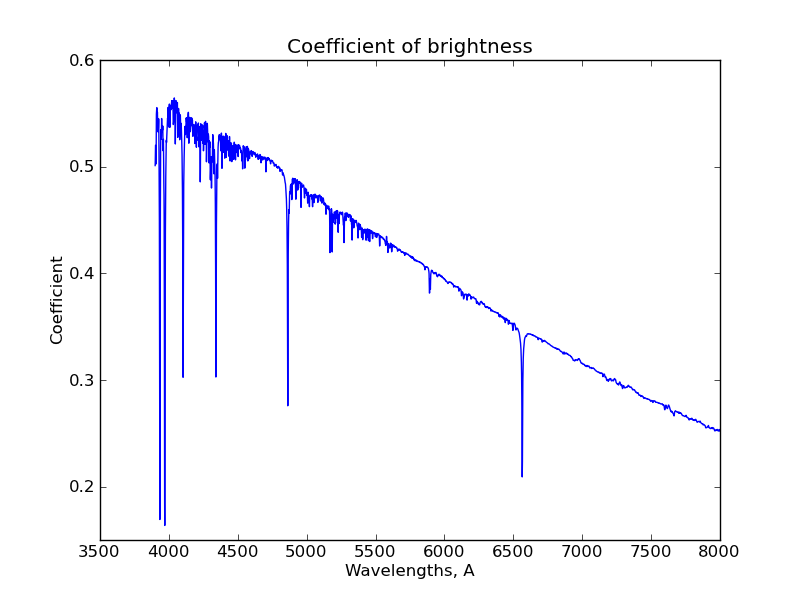
\includegraphics[width=12cm]{../coeffs0}\\
\caption{Coefficients of brightness as a function of wavelength}
\end{figure}
\begin{figure}
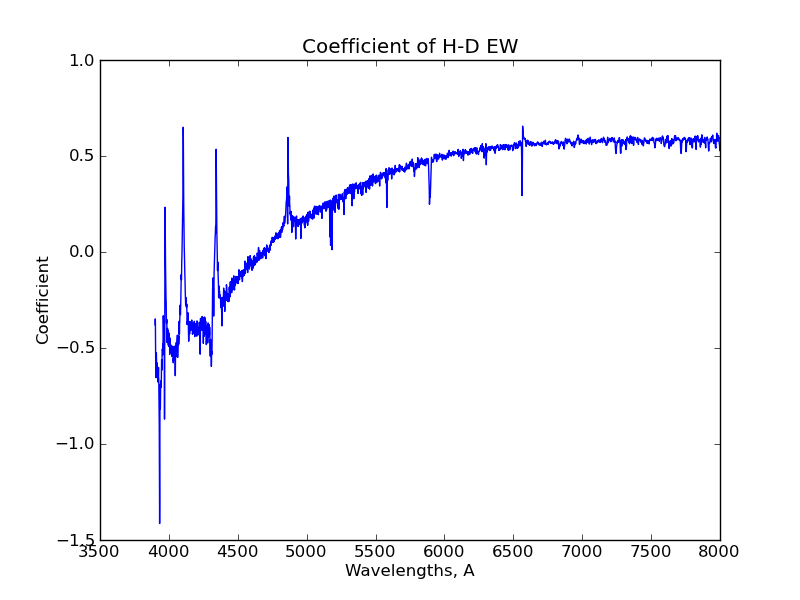
\includegraphics[width=12cm]{../coeffs1}\\
\caption{Coefficients of H-$\delta$ as a function of wavelength}
\end{figure}
\begin{figure}
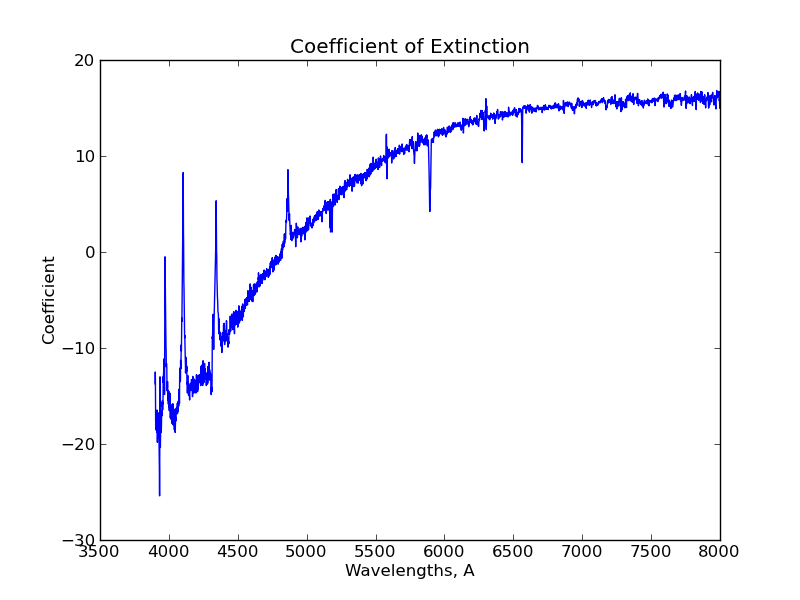
\includegraphics[width=12cm]{../coeffs2}\\
\caption{Coefficients of extinction as a function of wavelength}
\end{figure}
\begin{figure}
\plottwo{../residuals8000.png}{../residuals.png}
\caption{Plot of expected flux values using the coefficients, and the actual flux values at 8000$\AA$.}
\end{figure}

\subsection{Changing to a non-linear model}
-The same process from above was repeated, but with a more physically-sound, non-linear model:\\
Observed flux = (a$\times$Brightness + b$\times$H-$\delta$ EW) $\times$ e$^{c \times Extinction}$\\
- This linearized the extinction variable.
\begin{figure}
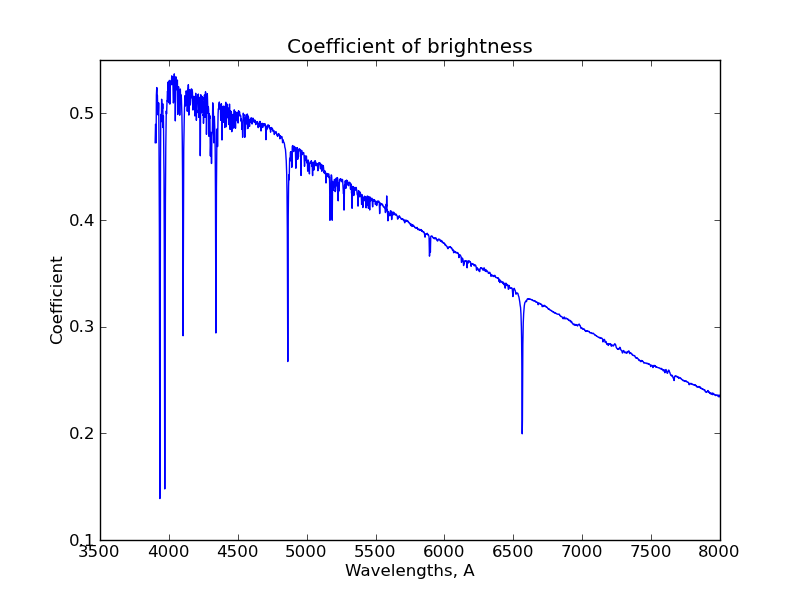
\includegraphics[width=12cm]{../coeffsdr9experr0}\\
\caption{Coefficients of brightness as a function of wavelength}
\end{figure}
\begin{figure}
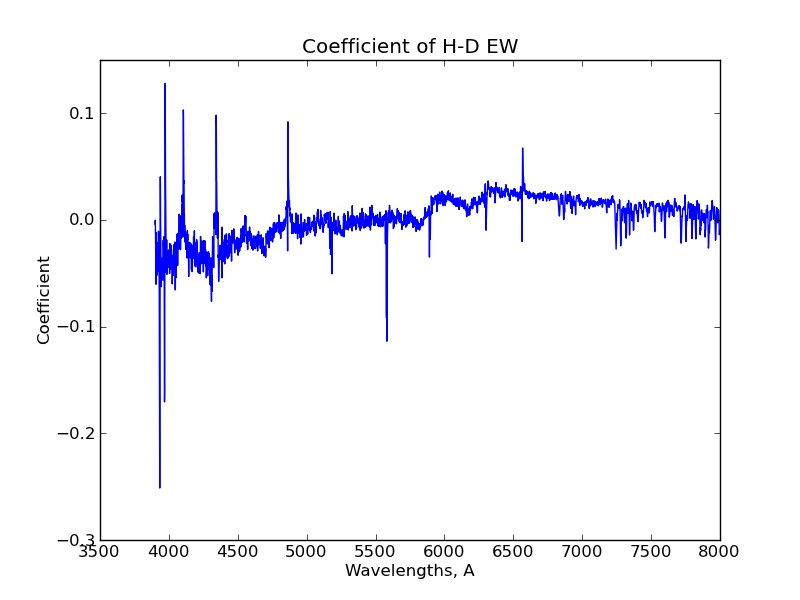
\includegraphics[width=12cm]{../coeffsdr9experr1}\\
\caption{Coefficients of H-$\delta$ as a function of wavelength}
\end{figure}
\begin{figure}
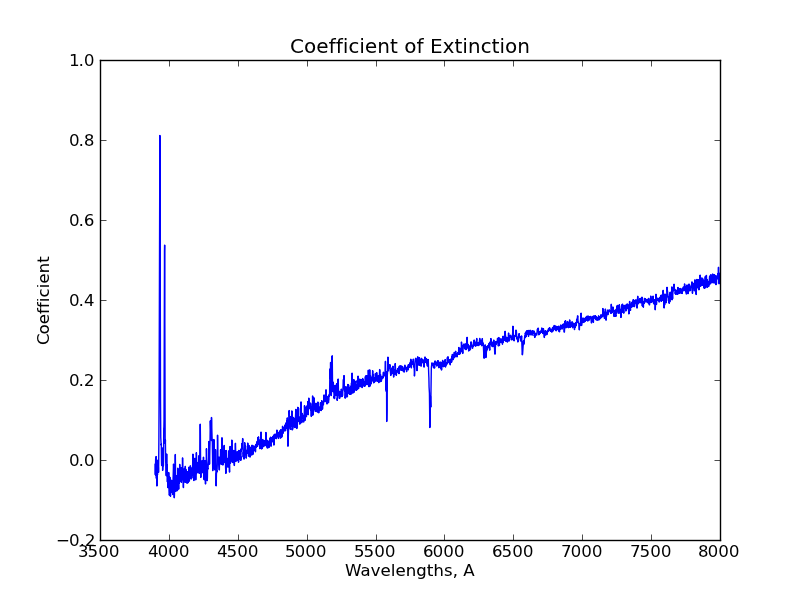
\includegraphics[width=12cm]{../coeffsdr9experr2}\\
\caption{Coefficients of extinction as a function of wavelength}
\end{figure}

\section{Discussion}
\subsection{Comparison with existing model (Whittet, Schlegel)}
- Table 3.1 (Whittet 1992) gives a list of values for A$_\lambda$/A$_V$, while Schlegel lists an A/A$_g$ value of 1.161 for the g-band. Combining the two gives a method to generate A/A$_g$ values, which were plotted against the coefficients obtained from our fit.
\begin{figure}
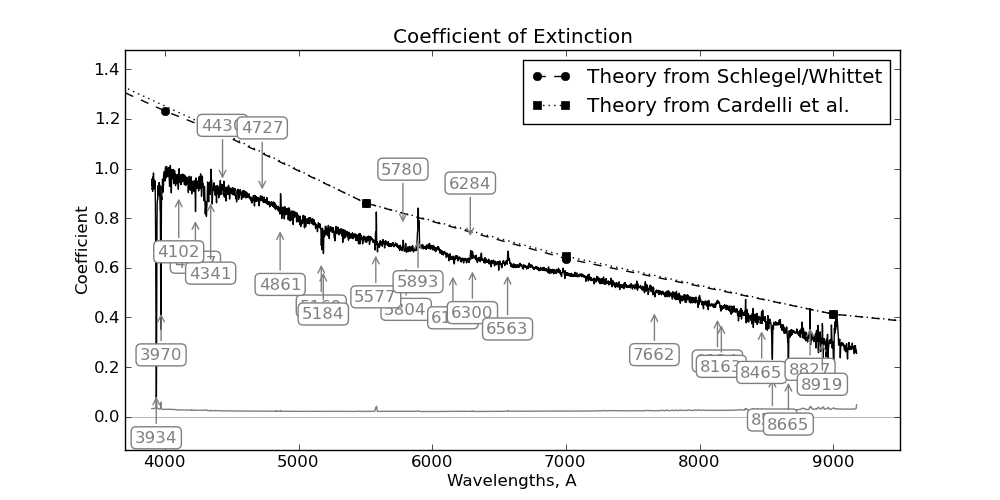
\includegraphics[width=12cm]{../test_curvefit_coefficients_ivar2}\\
\caption{Coefficients of extinction plotted against known values from Whittet and Schlegel and Cardelli et al.}
\end{figure}


\end{document}
